\section{Design of \TOOL}
\label{section:design}

%------------------------------------------------------------------------------
\myparagraphsquish{Problem Definition.}
%
Given the features of the SGX, a client's enclave is opaque to the cloud
provider. This benefits clients because it protects the confidentiality and
integrity of their sensitive content. However, the cloud provider can no longer
inspect or enforce any policies on enclave content.

In this paper, we remedy the situation by introducing \tool, which statically
checks the policy compliance of the code that the client proposes to execute in
its enclaves. The client and cloud provider agree upon a set of policies that
the client's code must satisfy. For instance, the cloud provider may require
the client to instrument its code with certain security checks or link its code
against certain versions of libraries. \tool's architecture supports plugging
in \textit{policy modules}, which check compliance based upon the policies that
the cloud provider and client mutually agree upon. \tool\ executes during
enclave provisioning, and checks that the client's enclave code is
policy-compliant. If the client's code is not policy compliant, \tool\ informs
the cloud provider, who can prevent code from executing.

%------------------------------------------------------------------------------
\myparagraph{Threat Model.} 
%
We assume that the cloud provider and client are mutually distrusting. Before
allowing the client to create and provision enclaves, the cloud provider and
client mutually agree upon the set of policies that the client's code must
satisfy. We assume that the code of \tool\ and its policy modules is available
to both the cloud provider and client for inspection. 

From the cloud provider's perspective, the client will attempt to violate the
mutually agreed-upon policies. It therefore verifies that \tool\ and its policy
modules indeed enforce these policies. From the client's perspective, the cloud
provider will attempt to learn the contents of the enclave. Thus, the client
verifies that \tool\ and its policy modules leak no additional information
about its code to the cloud provider, \ie~the only explicit communication
between \tool\ and the cloud provider must be to inform the cloud provider
about policy compliance and to identify the virtual addresses of the pages that
contain the client's code. For this paper, we do not consider implicit and
covert communication channels via which \tool\ can communicate information
about the client's code to the cloud provider; techniques to analyze \tool's
code for such covert channels can be the subject of future research. The client
can also use \tool\ to independently verify policy compliance of the enclave
code that it wants to provision.

Both the cloud provider and the client trust the SGX hardware platform. \tool\
and its policy modules are loaded into a freshly-created enclave (as part of
the bootstrap code). Both the provider and the client use SGX's attestation
features to ensure that \tool\ was correctly loaded into the enclave. \tool\
receives the client code over a SSL/TLS channel, checks policy compliance, and
informs the cloud provider. Any attempts by the cloud provider to cheat, \eg~by
falsely claiming that the code is not policy-compliant or failing to allow
policy-compliant code to execute, can easily be detected by the client.

%------------------------------------------------------------------------------

%%%%%

\myparagraph{Overall Design.} 
%
\tool\ primarily consists of in-enclave components that are loaded when an
enclave is created (see \figref{figure:overalldesign}). As is standard on all
SGX systems, the client first ensures (using SGX's attestation
protocols~\cite{sgx:attest:hasp13}) that the enclave was initialized securely.

Following this step, the client sets up an end-to-end encrypted channel with
the enclave. To do this, the bootstrap code loaded into a freshly-created
enclave first generates a 2048-bit RSA key pair and then establishes a socket
connection to the client machine. As a next step, the enclave sends its
newly-generated public key to the client machine so that it can encrypt its
256-bit AES key and sends the encrypted AES key back to the loader. This key is
used to establish an end-to-end encrypted channel with the client.

\begin{wrapfigure}{lt}{1.65in}
\centering
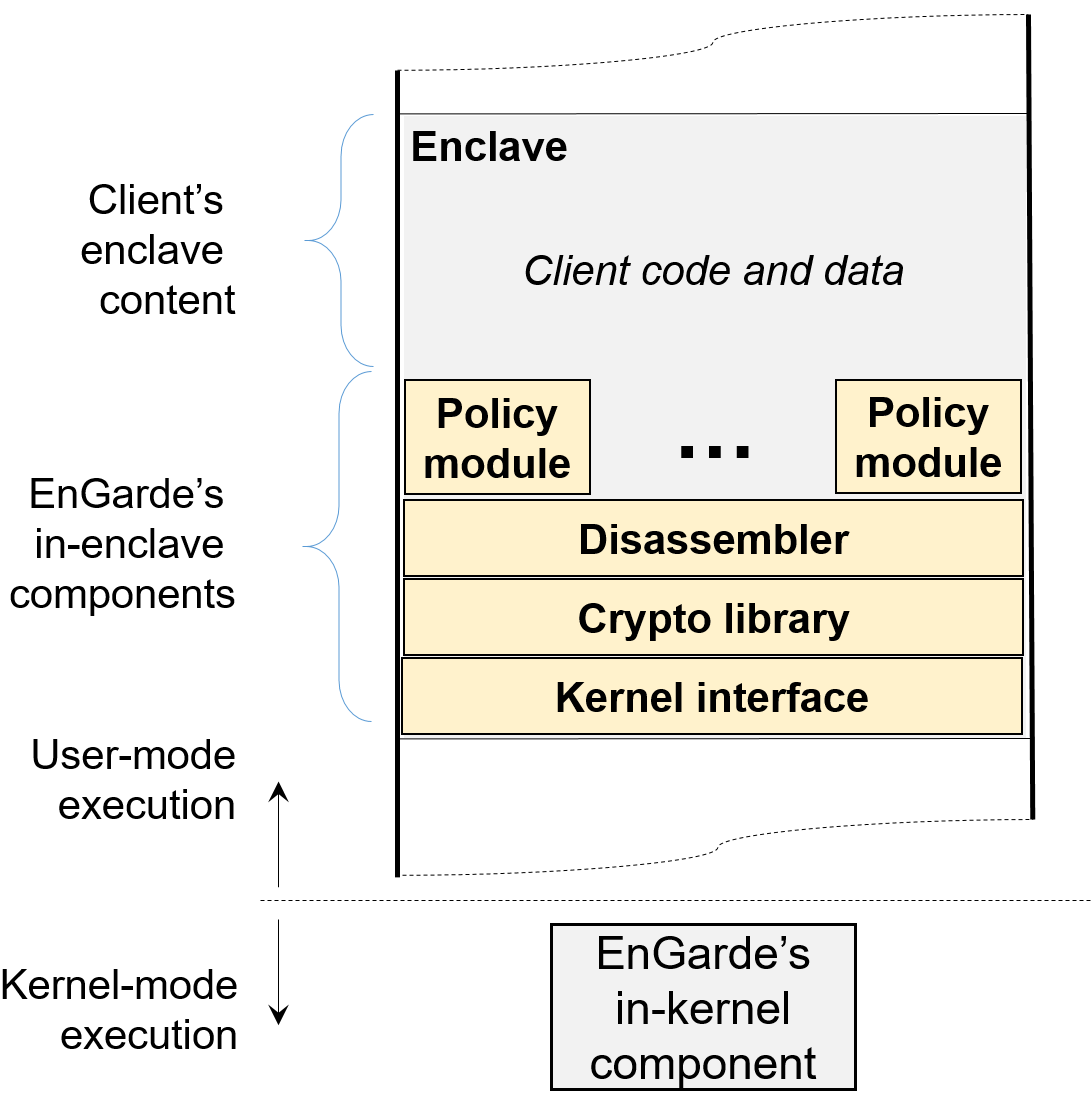
\includegraphics[keepaspectratio=true,width=0.25\textwidth]{figures/engarde.png}
\indent\vspace{-0.3cm}
\mycaption{Design of \tool.}{\label{figure:overalldesign}}
\indent\vspace{-0.7cm}
\end{wrapfigure}

\tool\ checks the client's enclave contents for policy compliance after the
client sends it the contents, but before the content is provisioned within the
enclave for execution. The client sends the content in encrypted blocks, which
\tool's crypto library decrypts to form an in-memory executable representation.

\tool\ operates at the granularity of memory pages, and therefore
splits the content into page-level chunks.  We assume that the client sends x86
binary code and identifies pages which contain code. The remaining pages are
assumed to contain data. \tool\ rejects pages that contain mixed code and data.
We assume that clients suitably compile their code so as to satisfy this
assumption. We also assume that the enclave code is not obfuscated to hinder
analysis.

Once \tool\ has received all the code, it proceeds to disassemble the client's
code. To do this, \tool\ relies on the disassembler provided by Google's Native
Client (NaCl)~\cite{nativeclient:oak09}. NaCl makes a number of assumptions to
ensure clean, unambiguous disassembly. For example, it requires no instructions
to overlap a 32-byte boundary, that all control-transfers target valid
instructions, and that all valid instructions are reachable from the start
address. \tool\ requires the client's enclave to satisfy the same constraints.

After disassembling the code, \tool\ checks the code for policy compliance.
Recall that the specific policies that \tool\ checks depend on those negotiated
with the client. In general, the policies can check structural properties of
the code, \eg~that certain instrumentation has been added to the code. \tool\
checks policies using pluggable \textit{policy modules}. Each policy module
checks compliance for a specific property, and specific policy modules that are
loaded during enclave creation depend upon the policies that the client and
cloud provider have agreed upon. In \sectref{section:evaluation}, we discuss
three examples of policy modules that we have implemented in our current \tool\
prototype. While \tool's disassembler works even on stripped binary code
(\ie~code without symbol-table information), specific policy modules may
require symbol table information to check compliance. If \tool's policy modules
require such information, then it requires the client to produce code using
symbol tables.

The policy modules determine whether the client's code is policy compliant. If
not, the code is rejected, and the enclave is not provisioned. If \tool\
determines that the code is policy-compliant, it then informs the host. \tool\
also contains a host-level component, either running within the host's OS
kernel or the hypervisor (if the host is virtualized). \tool's in-enclave
components provide the in-kernel component with a list of executable code
pages. The underlying OS component marks these pages as executable, but not
writable. The remaining pages are given write permissions, but are not given
execute permissions. The host OS component of \tool\ also prevents the enclave
from being extended after it has been provisioned. This ensures that the client
cannot inject any further code into the enclave after it has been checked for
compliance. \tool's in-kernel component enforces execute and write permissions
by setting page-table permission bits in the underlying host OS. While the
current version of SGX hardware allows for page permissions to be set/cleared
by the host OS, it does not yet offer support for page permissions at the
hardware level (\ie~page permissions for EPC pages). This feature has been
proposed in version~2 of the SGX instruction set~\cite{sgx:v2:na}. Although
\tool\ can be implemented readily  even on SGX version~1 processors, the
permission check can only be enforced in software within the host OS, and this
has been shown to be open to attack~\cite{asyncshock:esorics16}. Thus, \tool\
requires the features of SGX version~2 for security.

Following this, the enclave can be accessed and executed as on traditional SGX
platforms. Note that \tool\ only operates during enclave provisioning. Thus,
\tool\ only imposes a performance penalty during enclave provisioning. Enclave
execution incurs no additional runtime overhead.

